\de{ĐỀ THI HK1 NĂM HỌC 2022-2023}{ TRƯỜNG THPT ĐÔ LƯƠNG 1 - NGHỆ AN}



\begin{center}
	\textbf{PHẦN 1 - TRẮC NGHIỆM}
\end{center}
\Opensolutionfile{ans}[ans/ans]
\setcounter{ex}{0}

\begin{ex}%[0D2B2-3]%[Dự án Đề Kiểm tra Toán 10-TinDatTran]%[Đô Lương 1-Nghệ An]
 Một đề thi cuối kỳ 1 gồm 35 câu hỏi trắc nghiệm và 3 bài tự luận. Khi làm đúng mỗi câu trắc
nghiệm sẽ được 0,2 điểm, làm đúng mỗi câu tự luận được 1 điểm. Giả sử bạn An làm đúng $x$ câu hỏi trắc
nghiệm và $y$ bài tự luận. Viết một bất phương trình bậc nhất hai ẩn $x$ và $y$ để đảm bảo bạn An được ít nhất $8$ điểm
\choice
{$0{,}2 x+y<8$}
{$x+0{,}2 y \geq 8$}
{\True $0{,}2 x+y \geq 8$}
{$35 x+3 y \geq 8$}
\loigiai{
Để bạn An được ít nhất $8$ điểm thì ta có bất phương trình $0{,}2x+y\geq 8$.
}
\end{ex}
\begin{ex}%[0D1B1-5]%[Dự án Đề Kiểm tra Toán 10-TinDatTran]%[Đô Lương 1-Nghệ An]
Phát biểu mệnh đề phủ định của mệnh đề ``$\forall n \in\mathbb{N} : n^2-5 n+9 \neq 0$''.
\choice
{``$\exists n \in\mathbb{N} : n^2-5 n+9 \leq 0$''}
{\True ``$\exists n \in\mathbb{N} : n^2-5 n+9=0$''}
{``$\exists n \in\mathbb{N} : n^2-5 n+9 \geq 0$''}
{``$\exists n \in\mathbb{N} : n^2-5 n+9 \neq 0$''}
\loigiai{
Mệnh đề phủ định của mệnh đề ``$\forall n \in\mathbb{N} : n^2-5 n+9 \neq 0$'' là ``$\exists n \in\mathbb{N} : n^2-5 n+9=0$''.
}
\end{ex}
\begin{ex}%[0H1Y2-1]%[Dự án Đề Kiểm tra Toán 10-TinDatTran]%[Đô Lương 1-Nghệ An]
Cho tam giác $ABC$. Khẳng định nào sau đây công thức \textbf{sai}?
\choice
{$\sin A=\dfrac{a}{2 R}$}
{$\dfrac{a}{\sin A}=2 R$}
{\True $b \sin B=2 R$}
{$\sin C=\dfrac{c \sin A}{a}$}
\loigiai{
Theo định lý Sin ta có
\[\dfrac{a}{\sin A}=\dfrac{b}{\sin B}=\dfrac{c}{\sin C}=2R\]
nên khẳng định  $b \sin B=2 R$ là công thức sai.
}
\end{ex}
\begin{ex}%[0X1Y3-1]%[0X1Y3-3]%[Dự án Đề Kiểm tra Toán 10-TinDatTran]%[Đô Lương 1-Nghệ An]
Cho mẫu số liệu sau
\begin{center}
	\begin{tabular}{c c c c c}
	156&158&160&162&164\\
\end{tabular}
\end{center}
Nếu bổ sung hai giá trị 154 và 167 vào mẫu số liệu thì so với mẫu ban đầu
\choice
{\True Trung vị không thay đổi, số trung bình thay đổi}
{Trung vị thay đổi, số trung bình không thay đổi}
{Trung vị và số trung bình đều thay đổi}
{Trung vị và số trung bình đều không thay đổi}
\loigiai{
Trung vị của mẫu ban đầu là $160$, số trung bình cộng của mẫu ban đầu là \[\dfrac{156+158+160+162+164}{5}=160.\]
Khi thêm hai giá trị $154$ và $160$ vào mẫu số liệu và sắp xếp thứ tự, ta được mẫu số liệu sau
\begin{center}
	\begin{tabular}{c c c c c c c}
		154 &156&158&160&162&164&167\\
	\end{tabular}
\end{center}
Trung vị của mẫu lúc sau là 160, số trung bình cộng của mẫu lúc sau là 
 \[\dfrac{154+156+158+160+162+164+167}{7}\approx 160{,}14.\]
Vậy trung vị không thay đổi, số trung bình thay đổi.
}
\end{ex}
\begin{ex}%[0H2B1-2]%[Dự án Đề Kiểm tra Toán 10-TinDatTran]%[Đô Lương 1-Nghệ An]
Cho hình chữ nhật $ABCD$. Có bao nhiêu vectơ khác $\overrightarrow{0}$ cùng phương với $\overrightarrow{AB}$ có điểm đầu và cuối là các đỉnh của hình chữ nhật?
\choice
{$1$}
{$3$}
{\True $4$}
{$2$}
\loigiai{
\immini{Các véc-tơ cùng phương với $\overrightarrow{AB}$ là $\overrightarrow{AB}$, $\overrightarrow{BA}$, $\overrightarrow{CD}$, $\overrightarrow{DC}$.}
{\begin{tikzpicture}
\path (0,0) coordinate (D)
(4,0) coordinate (C)
(0,3) coordinate (A)
(4,3) coordinate (B);
\draw (A)--(B)--(C)--(D)--cycle;
\foreach \t/\g in {A/135,B/45,C/-45,D/-135}{
	\draw[fill=white] (\t) circle (1pt) node[shift={(\g:7pt)},font=\scriptsize]{$ \t $};
}
\end{tikzpicture}}
}
\end{ex}
\begin{ex}%[0H3K1-4]%[Dự án Đề Kiểm tra Toán 10-TinDatTran]%[Đô Lương 1-Nghệ An]
Trong mặt phẳng tọa độ $Oxy$, cho hai điểm $A(2 ;-4)$ và $B(10 ; 4)$. Gọi $C$ là giao điểm của đường thẳng $AB$ với trục hoành. Đặt $\overrightarrow{AB}=k \cdot \overrightarrow{AC}$, giá trị của $k$ là:
\choice
{\True $2$}
{$-\dfrac{1}{2}$}
{$\dfrac{1}{2}$}
{$-2$}
\loigiai{
Gọi $C(x;0)$ là giao điểm của $AB$ với trục hoành. Ta có $\overrightarrow{AB}=(8;8)$, $\overrightarrow{AC}=(x-2;4)$. Vì $A$, $B$, $C$ thẳng hàng nên
\[\dfrac{x-2}{8}=\dfrac{4}{8}\Leftrightarrow x=6\Rightarrow \overrightarrow{AC}=(4;4).\]
Khi đó $\overrightarrow{AB}=2\overrightarrow{AC}$.
}
\end{ex}
\begin{ex}%[0H2K2-6]%[Dự án Đề Kiểm tra Toán 10-TinDatTran]%[Đô Lương 1-Nghệ An]
Một chiếc tàu di chuyển theo hướng Bắc với vận tốc riêng $25$km/h, dòng nước chảy theo hướng Đông với vận tốc $3$km/h. Hỏi tàu di chuyển với vận tốc thực tế là bao nhiêu? (làm tròn đến hàng phần chục)
\choice
{$25{,}1~\mathrm{km/h}$}
{$22~\mathrm{km/h}$}
{$28~\mathrm{km/h}$}
{\True$25{,}2~\mathrm{km/h}$}
\loigiai{
\begin{center}
\begin{tikzpicture}[line join=round,line cap=round,>=stealth]
	\path (0,0) coordinate (O)
	(0,4) coordinate (A)
	(2,0) coordinate (B)
	(2,4) coordinate (C)
	;
	\draw[->] (O)--(A)node[right]{$\vec{v}_{\text{tàu}}$};
	\draw[->] (O)--(B)node[above]{$\vec{v}_{\text{nước}}$};
	\draw[->] (O)--(C)node[right]{$\vec{v}_{\text{thực tế}}$};
\end{tikzpicture}
\end{center}
Vận tốc thực tế của tàu là $\sqrt{25^2+3^2}\approx25{,}2$km/h.
}
\end{ex}
\begin{ex}%[0H2Y4-3]%[Dự án Đề Kiểm tra Toán 10-TinDatTran]%[Đô Lương 1-Nghệ An]
Khẳng định nào sau đây đúng?
\choice
{$(\vec{a} \cdot \vec{b}) \cdot \vec{c}=\vec{a} \cdot(\vec{b} \cdot \vec{c})$}
{$\vec{a} \cdot \vec{b}=|\vec{a}| \cdot|\vec{b}| \sin (\vec{a} ; \vec{b})$}
{\True $\vec{a} \cdot(\vec{b}+\vec{c})=\vec{a} \cdot \vec{b}+\vec{a} \cdot \vec{c}$}
{$(\vec{a} \cdot \vec{b})^2=\vec{a}^2 \cdot \vec{b}^2$}
\loigiai{
Trong các khẳng định trên, khẳng định $\vec{a} \cdot(\vec{b}+\vec{c})=\vec{a} \cdot \vec{b}+\vec{a} \cdot \vec{c}$ là khẳng định đúng.
}
\end{ex}
\begin{ex}%[0X1Y4-3]%[Dự án Đề Kiểm tra Toán 10-TinDatTran]%[Đô Lương 1-Nghệ An]
Số đặc trưng nào sau đây đo độ phân tán của mẫu số liệu?
\choice
{Số trung bình}
{\True Phương sai}
{Trung vị}
{Mốt}
\loigiai{Phương sai đo độ phân tán của mẫu số liệu.}
\end{ex}
\begin{ex}%[0D1B2-3]%[Dự án Đề Kiểm tra Toán 10-TinDatTran]%[Đô Lương 1-Nghệ An]
Dùng các kí hiệu khoảng, đoạn, nửa khoảng viết lại tập hợp \[A=\{x \in \mathbb{R} \mid 1 \leq x \leq 2\}.\]
\choice
{\True $[1 ; 2]$}
{$[1 ; 2)$}
{$\{1 ; 2\}$}
{$(1 ; 2)$}
\loigiai{
Ta có $A=\{x \in \mathbb{R} \mid 1 \leq x \leq 2\}=[1;2]$.
}
\end{ex}
\begin{ex}%[0H3Y1-3]%[Dự án Đề Kiểm tra Toán 10-TinDatTran]%[Đô Lương 1-Nghệ An]
Trong mặt phẳng với hệ trục tọa độ $Oxy$, Cho 3 điểm $A(-3 ; 1)$, $B(2 ;-1)$, $C(4 ; 6)$. Tọa độ trọng tâm $G$ của tam giác $ABC$ là
\choice
{$(1 ;-2)$}
{\True $(1 ; 2)$}
{$(2 ; 1)$}
{$(-2 ; 1)$}
\loigiai{
Tọa độ trọng tâm $G$ của tam giác $ABC$ là $\left(\dfrac{-3+2+4}{3};\dfrac{1+(-1)+6}{3}\right)=(1;2)$
}
\end{ex}
\begin{ex}%[0D2Y1-1]%[Dự án Đề Kiểm tra Toán 10-TinDatTran]%[Đô Lương 1-Nghệ An]
Bất phương trình nào sau đây không phải là bất phương trình bậc nhất hai ẩn?
\choice
{\True $x+y^2 \geq 2$}
{$2(y+x) \leq 3(x+1)$}
{$3 x-y \geq 5$}
{$x+y \leq 0$}
\loigiai{
Bất phương trình $x+y^2 \geq 2$ không phải là bất phương trình bậc nhất hai ẩn.
}
\end{ex}
\begin{ex}%[0H3Y2-1]%[Dự án Đề Kiểm tra Toán 10-TinDatTran]%[Đô Lương 1-Nghệ An]
Góc giữa véc-tơ $\vec{a}(2 ; 1)$ và véc-tơ $\vec{b}(3 ;-1)$ có số đo bằng:
\choice
{$135^\circ$}
{$150^\circ$}
{\True $45^\circ$}
{$60^\circ$}
\loigiai{
Ta có $\cos(\vec{a},\vec{b})=\dfrac{\vec{a}\cdot \vec{b}}{|\vec{a}|\cdot |\vec{b}|}=\dfrac{2\cdot 3+1\cdot (-1)}{\sqrt{2^2+1}\cdot \sqrt{3^2+(-1)^2}}=\dfrac{\sqrt{2}}{2}\Rightarrow(\vec{a},\vec{b})=45^\circ$.
}
\end{ex}
\begin{ex}%[0X1B3-2]%[Dự án Đề Kiểm tra Toán 10-TinDatTran]%[Đô Lương 1-Nghệ An]
Chỉ số IQ của một nhóm 11 học sinh:
\begin{center}
\begin{tabular}{c c c c c c c c c c c}
	60&72&63&83&68&90&74&86&74&80&82\\
\end{tabular}
\end{center}
Tìm trung vị của mẫu số liệu vừa cho
\choice
{77}
{68}
{73}
{\True 74}
\loigiai{
Sắp xếp thứ tự mẫu số liệu vừa cho ta được bảng số liệu sau
\begin{center}
\begin{tabular}{c c c c c c c c c c c}
60&63&68&72&74&74&80&82&83&86&90\\
\end{tabular}
\end{center}
Trung vị của mẫu số liệu trên là $74$.
}
\end{ex}
\begin{ex}%[0D1Y1-1]%[Dự án Đề Kiểm tra Toán 10-TinDatTran]%[Đô Lương 1-Nghệ An]
Phát biểu nào sau đây là một mệnh đề?
\choice
{\True FIFA World cup 2022 là giải vô địch bóng đá thế giới lần thứ 22}
{FIFA World cup 2026 có mấy quốc gia đồng tổ chức?}
{Ôi, bàn thắng của Lionel Messi thật đẳng cấp!}
{Bạn có thích xem bóng đá không?}
\loigiai{
Trong các phát biểu trên, phát biểu ``FIFA World cup 2022 là giải vô địch bóng đá thế giới lần thứ 22'' là một mệnh đề.
}
\end{ex}
\begin{ex}%[0D1B3-4]%[Dự án Đề Kiểm tra Toán 10-TinDatTran]%[Đô Lương 1-Nghệ An]
Cho hai tập hợp $A=[-2 ; 3]$ và $B=(1 ;+\infty)$. Khẳng định nào sau đây đúng?
\choice
{$A \cap B=(-2 ; 1)$}
{\True $A \cap B=(1 ; 3]$}
{$A \cap B=[1 ; 3]$}
{$A \cap B=[-2 ;+\infty)$}
\loigiai{
Ta có $A \cap B=(1 ; 3]$.
}
\end{ex}
\begin{ex}%[0X1B3-4]%[Dự án Đề Kiểm tra Toán 10-TinDatTran]%[Đô Lương 1-Nghệ An]
Số đường chuyền tạo cơ hội của siêu sao Lionel Messi trong mỗi trận đấu tại World Cup 2022 như sau
\begin{center}
	\begin{tabular}{c c c c c c c c c c c c c c}
		18&19&17&21&22&21&18&19&21&20&23&18&21&20\\
	\end{tabular}
\end{center}
Mốt của mẫu số liệu trên là:
\choice
{\True 21}
{19}
{18}
{20}
\loigiai{
Mốt của mẫu số liệu trên là $21$.
}
\end{ex}
\begin{ex}%[0H1B1-2]%[Dự án Đề Kiểm tra Toán 10-TinDatTran]%[Đô Lương 1-Nghệ An]
Cho góc $\alpha$ thỏa mãn $\sin \alpha=\dfrac{5}{13},\left(90^\circ<\alpha<180^\circ\right)$. Giá trị của $\cos \alpha$ là
\choice
{$-\dfrac{8}{13}$}
{\True $-\dfrac{12}{13}$}
{$\dfrac{8}{13}$}
{$\dfrac{12}{13}$}
\loigiai{
Vì $90^\circ<\alpha<180^\circ$ nên $\cos \alpha <0$.\\
Ta có $\cos\alpha=\sqrt{1-\sin^2\alpha}=\sqrt{1-\left(\dfrac{5}{13}\right)^2}=-\dfrac{12}{13}$ (vì $\cos \alpha <0$).
}
\end{ex}


%Câu 18
\begin{ex}%[0T4B1-2]%[Dự án đề kiểm tra HKI NH22-23- Phạm Văn Long]%[THPT Đô Lương 1 Nghệ An]
   Cho góc $\alpha$ thỏa mãn $\sin \alpha = \dfrac{5}{13}$ $(90^\circ < \alpha < 180^\circ)$. Giá trị của $\cos \alpha$ là
   \choice
   {$-\dfrac{8}{13}$}
   {\True $-\dfrac{12}{13}$}
   {$\dfrac{8}{13}$}
   {$\dfrac{12}{13}$}
   \loigiai{
      Ta có 
      \[\cos^2 \alpha = 1-\sin^2 \alpha = 1-\left(\dfrac{5}{13}\right)^2 = \dfrac{144}{169}\Leftrightarrow \hoac{&\cos \alpha = \dfrac{12}{13}\\&\cos \alpha =-\dfrac{12}{13}.}\]
      Vì $90^\circ < \alpha < 180^\circ$ nên $\cos \alpha <0$.\\
      Vậy $\cos \alpha = -\dfrac{12}{13}$.
   }
\end{ex}

%Câu 19
\begin{ex}%[0T5B4-1]%[Dự án đề kiểm tra HKI NH22-23- Phạm Văn Long]%[THPT Đô Lương 1 Nghệ An]
   Cho hình vuông $ABCD$ có cạnh bằng $a$. Khẳng định nào sau đây đúng?
   \choice
   {$\left(\overrightarrow{AD}, \overrightarrow{CA}\right)=45^\circ$}
   {\True $\overrightarrow{AB} \cdot \overrightarrow{BD} = a^2$}
   {$\overrightarrow{AC} \cdot \overrightarrow{DB} = 2a^2$}
   {$\overrightarrow{AB} \cdot \overrightarrow{DB} = a^2$}
   \loigiai{
      \immini{
      Ta có 
      \allowdisplaybreaks
      \begin{eqnarray*}
      \overrightarrow{AB}\cdot \overrightarrow{DB} = \overrightarrow{DC}\cdot \overrightarrow{DB}  
      &=& \left|\overrightarrow{DC}\right| \cdot \left|\overrightarrow{DB}\right| \cdot \cos \left(\overrightarrow{DB},\overrightarrow{DC}\right)\\
      &=&a\sqrt{2}\cdot a\cdot \cos 45^\circ\\
      &=&a^2.
      \end{eqnarray*}
      }{
         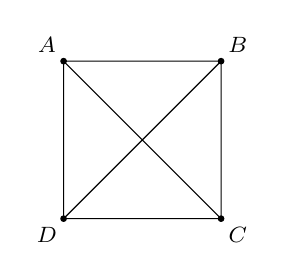
\begin{tikzpicture}[>=stealth,line join=round,line cap=round,font=\footnotesize,scale=1]
            \def\a{2}
            \draw 
               (0,0) coordinate (A)
               (\a,0) coordinate (B)
               (\a,-\a) coordinate (C)
               (0,-\a) coordinate (D)
            ;
            \draw (A)--(B)--(C)--(D)--cycle (C)--(A) (B)--(D);
            \foreach \l/\g in {A/135,B/45,C/-45,D/-135}
               \draw[fill=black] (\l) circle (1pt) +(\g:.3) node{$\l$};
         \end{tikzpicture}
      }
   }
\end{ex}

%Câu 20
\begin{ex}%[0T5B4-1]%[Dự án đề kiểm tra HKI NH22-23- Phạm Văn Long]%[THPT Đô Lương 1 Nghệ An]
   Cho $\overrightarrow{a}$ và $\overrightarrow{b}$ là hai véc-tơ ngược hướng và đều khác véc-tơ $\overrightarrow{0}$. Mệnh đề nào sau đây đúng?
   \choice
   {$\overrightarrow{a}\cdot \overrightarrow{b}=0$}
   {\True $\overrightarrow{a}\cdot \overrightarrow{b}=-\left|\overrightarrow{a}\right|\cdot\left|\overrightarrow{b}\right|$}
   {$\overrightarrow{a}\cdot \overrightarrow{b}= \left|\overrightarrow{a}\right|\cdot\left|\overrightarrow{b}\right|$}
   {$\overrightarrow{a}\cdot\overrightarrow{b}= -1$}
   \loigiai{
      Ta có $\overrightarrow{a}\cdot \overrightarrow{b} = \left|\overrightarrow{a}\right|\cdot \left|\overrightarrow{b}\right|\cos 180^\circ = -\left|\overrightarrow{a}\right|\cdot \left|\overrightarrow{b}\right|$.
   }
\end{ex}

%Câu 21
\begin{ex}%[0T6B1-1] %[Dự án đề kiểm tra HKI NH22-23- Phạm Văn Long]%[THPT Đô Lương 1 Nghệ An]
   Đo vận tốc trung bình của một chiếc xe ô tô chạy trên đường cao tốc, ta được kết quả là $v=100\pm 5$ (km/h). Mệnh đề nào \textbf{sai}?
   \choice
   {Sai số tương đối $\delta_v \leq \dfrac{5}{100}=5\%$}
   {Giá trị của $\overline{v}$ thuộc đoạn $[95;105]$}
   {\True Sai số tương đối $\delta_v = \dfrac{5}{100}=5\%$}
   {Độ chính xác $d=5$ km/h}
   \loigiai{
      Với $v = 100 \pm 5$ (km/h), ta có 
      \begin{itemize}
         \item Sai số tương đối $\delta_v \leq \dfrac{5}{100}=5\%$.
         \item Độ chính xác $d=5$ (km/h).
         \item Giá trị của $\overrightarrow{v}$ thuộc đoạn $[95;105]$.
      \end{itemize}
      
   }
\end{ex}

%Câu 22
\begin{ex}%[0T5B3-9]%[Dự án đề kiểm tra HKI NH22-23- Phạm Văn Long]%[THPT Đô Lương 1 Nghệ An]
   Cho hai lực $\overrightarrow{F_1}$, $\overrightarrow{F_2}$ không cùng phương, cùng tác dụng vào một vật, biết $\left|\overrightarrow{F_1}\right| = \left|\overrightarrow{F_2}\right| = 10$ N và $\left(\overrightarrow{F_1},\overrightarrow{F_2}\right)=60^\circ$. Độ lớn của hợp lực $\overrightarrow{F_1} + \overrightarrow{F_2}$ (làm tròn đến hàng phần trăm) bằng.
   \choice
   {$20$ N}
   {$14{,}1$ N}
   {$10$ N}
   {\True $17{,}3$ N}
   \loigiai{
      Ta có 
      \[\left(\overrightarrow{F_1} + \overrightarrow{F_2}\right)^2 = \overrightarrow{F_1}^2 + \overrightarrow{F_2}^2 + 2\overrightarrow{F_1}\cdot\overrightarrow{F_2} = 10^2 + 10^2 + 2\cdot 10\cdot 10\cdot\cos 60^\circ=300.\]
      Suy ra $\left| \overrightarrow{F_1} + \overrightarrow{F_2}\right| = 10\sqrt{3}\approx 17{,}3$ (N).
   }
\end{ex}

%Câu 23
\begin{ex}% [0T4B3-2]%[Dự án đề kiểm tra HKI NH22-23- Phạm Văn Long]%[THPT Đô Lương 1 Nghệ An]
   Hai chiếc tàu thủy cùng xuất phát từ vị trí $A$, đi thẳng theo hai hướng tạo với nhau một góc $60^\circ$. Tàu thứ nhất chạy với tốc độ $50$ km/h, tàu thứ hai chạy với tốc độ $60$ km/h. Hỏi sau $2$ giờ hai tàu cách nhau bao nhiêu km? (kết quả làm tròn đến hàng phần chục)
   \choice
   {\True $111{,}4$ km}
   {$110$ km}
   {$110{,}5$ km}
   {$112$ km}
   \loigiai{
      Ta có $AB = 50\cdot 2 =100$ km; $AC=60\cdot 2 =120$ km.
      Áp dụng định lý cosine, ta có
      \[BC^2 = AB^2 + AC^2 - 2AB\cdot AC \cdot \cos 60^\circ = 100^2 + 120^2 - 2\cdot 100\cdot 120\cdot\cos 60^\circ = 12400.\]
      Suy ra $BC = \sqrt{12400}\approx 111{,}4$ (km).\\
      Vậy sau $2$ giờ, hai tàu cách nhau khoảng $111{,}4$ km.
   }
\end{ex}

%Câu 24
\begin{ex}%[0T6B1-3]%[Dự án đề kiểm tra HKI NH22-23- Phạm Văn Long]%[THPT Đô Lương 1 Nghệ An]
   Làm tròn số $8316{,}2$ đến hàng chục. Khi đó số tuyệt đối của số quy tròn là
   \choice
   {$3{,}6$}
   {$6{,}2$}
   {$3{,}16$}
   {\True $3{,}8$}
   \loigiai{
      Số quy tròn của $\overline{a}=8316{,}2$ đến hàng chục là $a=8320$.\\
      Sai số tuyệt đối của số quy tròn là $\Delta a= \left|a-\overline{a}\right|=|8320 - 8216{,}2|= 3{,}8$.
   }
\end{ex}

%Câu 25
\begin{ex}%[0T9Y1-6]%[Dự án đề kiểm tra HKI NH22-23- Phạm Văn Long]%[THPT Đô Lương 1 Nghệ An]
   Trong mặt phẳng $Oxy$, cho hai véc-tơ $\overrightarrow{a}=(a_1;b_1)$ và $\overrightarrow{b} = \left(a_2;b_2\right)$. Mệnh đề nào sau đây đúng?
   \choice
   {$\overrightarrow{a}\cdot \overrightarrow{b} = a_1b_2 + a_2b_1$}
   {$\overrightarrow{a}\cdot \overrightarrow{b} = (a_1 + b_1)\left(a_2 + b_2\right)$}
   {$\overrightarrow{a}\cdot \overrightarrow{b} = a_1b_1 + a_2b_2$}
   {\True $\overrightarrow{a}\cdot \overrightarrow{b} = a_1a_2 + b_1b_2$}
   \loigiai{
      Ta có $\overrightarrow{a}\cdot\overrightarrow{b}=a_1a_2 + b_1b_2$.
   }
\end{ex}

%Câu 26
\begin{ex}%[0T9B1-3]%[Dự án đề kiểm tra HKI NH22-23- Phạm Văn Long]%[THPT Đô Lương 1 Nghệ An]
   Trong mặt phẳng tọa độ $Oxy$, cho hai điểm $A(1;5)$ và $B(8;4)$. Tìm tọa độ điểm $C$ thuộc trục tung sao cho $\triangle ABC$ vuông tại $A$.
   \choice
   {$C\left(0;-\dfrac{5}{2}\right)$}
   {$C(0;-3)$}
   {$C(0;2)$}
   {\True $C(0;-2)$}
   \loigiai{
      Vì $C\in Oy$ nên $C(0;a)$
      Ta có $\overrightarrow{AB} = (7;-1)$, $\overrightarrow{AC}=(-1;a-5)$.\\
      $\triangle ABC$ vuông tại $A$ khi và chỉ khi 
      \[\overrightarrow{AB}\cdot \overrightarrow{AC} = 0 \Leftrightarrow (-1)\cdot 7 + (-1)\cdot (a-5)=0 \Leftrightarrow a=-2.\]
      Vậy $C(0;-2)$.
   }
\end{ex}

%Câu 27
\begin{ex}%[0T9B1-7]%[Dự án đề kiểm tra HKI NH22-23- Phạm Văn Long]%[THPT Đô Lương 1 Nghệ An]
   Sự chuyển động của một tàu thủy được thể hiện trên một mặt phẳng tọa độ như sau: Tàu khởi hành từ vị trí $A(1;2)$ chuyển động thẳng đều với vận tốc (tính theo giờ) được biểu thị bởi véc-tơ $\overrightarrow{v} = (3;1)$. Tại thời điểm sau khi khởi hành $2$ giờ thì vị trí của tàu là điểm $B$ (trên mặt phẳng tọa độ) có tọa độ là
   \choice
   {\True $B(7;4)$}
   {$B(4;3)$}
   {$B(-5;0)$}
   {$B(5;5)$}
   \loigiai{
      Ta có $\overrightarrow{AB} = 2\overrightarrow{v} \Leftrightarrow \heva{&x_B - 1 = 2\cdot 3\\&y_B -2 = 2\cdot 1} \Leftrightarrow\heva{&x_B = 7\\&y_B = 4.}$\\
      Vậy $B(7;4).$
   }
\end{ex}

%Câu 28
\begin{ex}%[0T6B4-2]%[Dự án đề kiểm tra HKI NH22-23- Phạm Văn Long]%[THPT Đô Lương 1 Nghệ An]
   Thống kê số bàn thắng (goals) của Lionel Messi trong các mùa giải $2009-2010$ đến $2020-2021$ như sau
   \[47\qquad 53 \qquad 73 \qquad 60 \qquad 41 \qquad 58 \qquad 41 \qquad 54 \qquad 45 \qquad 51\qquad 31 \qquad 16\]
   Các giá trị bất thường (nếu có) trong mẫu số liệu trên là
   \choice
   {$73$}
   {$16$ và $73$}
   {$16$ và $31$}
   {\True $16$}
   \loigiai{
   Mẫu số liệu sắp xếp lại là 
   \[16\qquad 31 \qquad 41  \qquad 41 \qquad 45 \qquad 47 \qquad 51 \qquad 53 \qquad 54 \qquad 58 \qquad 60\qquad 73\]
   Tứ phân vị: $Q_1 = 41$, $Q_2=49$, $Q_3=56$.\\
   Khoảng tứ phân vị: $\Delta_Q = Q_3-Q_1=15$.\\
   \[Q_1 - 1{,}5\Delta_Q = 18{,}5;\quad Q_3 + 1{,}5\Delta_Q = 78{,}5.\]
   Vậy giá trị bất thường của mẫu số liệu là $16$.
   }
\end{ex}

%Câu 29
\begin{ex}%[0T5B3-1]%[Dự án đề kiểm tra HKI NH22-23- Phạm Văn Long]%[THPT Đô Lương 1 Nghệ An]
   Cho đoạn thẳng $AB$. Gọi $M$ là một điểm thuộc đoạn thẳng $AB$ sao cho $AM=\dfrac{1}{4}AB$. Khẳng định nào sau đây \textbf{sai}?
   \choice
   {$\overrightarrow{MB} = -3\overrightarrow{MA}$}
   {$\overrightarrow{AM} = \dfrac{1}{4}\overrightarrow{AB}$}
   {\True $\overrightarrow{MA} = \dfrac{1}{3}\overrightarrow{MB}$}
   {$\overrightarrow{BM} = \dfrac{3}{4}\overrightarrow{BA}$}
   \loigiai{
      \immini{
         Ta có khẳng định sai là \lq\lq$\overrightarrow{MA} = \dfrac{1}{3}\overrightarrow{MB}$\rq\rq.
      }
      {
      \begin{tikzpicture}[>=stealth,line join=round,line cap=round,font=\footnotesize,scale=1]
         \draw 
            (0,0) coordinate (A)
            (6,0) coordinate (B)
            ($(A)!1/3!(B)$) coordinate (M)
         ;
         \draw (A)--(B);
         \foreach \l/\g in {A/-90,M/90,B/-90}
            \draw[fill=black] (\l) circle (1pt) +(\g:.3) node{$\l$};
      \end{tikzpicture}
      }
   }
\end{ex}

%Câu 30
\begin{ex}%[0T5B4-2]%[Dự án đề kiểm tra HKI NH22-23- Phạm Văn Long]%[THPT Đô Lương 1 Nghệ An]
   Trong mặt phẳng với hệ trục tọa độ $Oxy$, cặp véc-tơ nào sau đây vuông góc với nhau?
   \choice
   {$\overrightarrow{u}=(1;-1)$ và $\overrightarrow{v} = (-1;1)$}
   {\True $\overrightarrow{u}=(4;3)$ và $\overrightarrow{v} = (3;-4)$}
   {$\overrightarrow{u}=(1;2)$ và $\overrightarrow{v} = (3;4)$}
   {$\overrightarrow{u}=(2;2)$ và $\overrightarrow{v}=(0;4)$}
   \loigiai{
      Với $\overrightarrow{u}=(4;3)$ và $\overrightarrow{v}=(3;-4)$, vì $4\cdot 3 + 3\cdot (-4)=0$ nên $\overrightarrow{u}\perp \overrightarrow{v}$.
   }
\end{ex}

%Câu 31
\begin{ex}%[0T4B1-1]%[Dự án đề kiểm tra HKI NH22-23- Phạm Văn Long]%[THPT Đô Lương 1 Nghệ An]
   Trong các khẳng định sau, khẳng định nào \textbf{sai}?
   \choice
   {$\cos 45^\circ = \sin 135^\circ$}
   {$\cos 45^\circ = \sin 45^\circ$}
   {\True $\cos 120^\circ = \sin 60^\circ$}
   {$\cos 30^\circ = \sin 120^\circ$}
   \loigiai{
      Khẳng định sai là \lq\lq$\cos 120^\circ = \sin 60^\circ$\rq\rq.
   }
\end{ex}

%Câu 32
\begin{ex}%[0T5B2-2]%[Dự án đề kiểm tra HKI NH22-23- Phạm Văn Long]%[THPT Đô Lương 1 Nghệ An]
   Cho ba điểm phân biệt $A$, $B$, $C$. Trong các khẳng định sau, khẳng định nào sau đây \textbf{sai}?
   \choice
   {$\overrightarrow{AC} + \overrightarrow{CB} = \overrightarrow{AB}$}
   {$\overrightarrow{CA} + \overrightarrow{BC} = \overrightarrow{BA}$}
   {\True $\overrightarrow{AB} - \overrightarrow{AC} = \overrightarrow{BC}$}
   {$\overrightarrow{AB} + \overrightarrow{BC} = \overrightarrow{AC}$}
   \loigiai{
      Khẳng định sai là \lq\lq$\overrightarrow{AB} - \overrightarrow{AC}=\overrightarrow{BC}$\rq\rq.
   }
\end{ex}

%Câu 33
\begin{ex}% [0T6B3-3]%[Dự án đề kiểm tra HKI NH22-23- Phạm Văn Long]%[THPT Đô Lương 1 Nghệ An]
   Tìm tứ phân vị thứ nhất của mẫu số liệu
   \[28\qquad 16\qquad 18 \qquad30 \qquad 19 \qquad 40 \qquad 100 \qquad 9 \qquad46 \qquad 10 \qquad 150 \qquad 200\]
   \choice
   {\True $17$}
   {$18$}
   {$16$}
   {$73$}
   \loigiai{
   Mẫu số liệu sắp xếp lại là 
   \[9\qquad 10 \qquad 16  \qquad 18 \qquad 19 \qquad 28 \qquad 30 \qquad 40 \qquad 46 \qquad 100 \qquad 150 \qquad 200.\]
   Tứ phân vị: $Q_1 = 17$, $Q_2=29$, $Q_3=73$.
   }
\end{ex}

%Câu 34
\begin{ex}%[0T4B2-1]%[Dự án đề kiểm tra HKI NH22-23- Phạm Văn Long]%[THPT Đô Lương 1 Nghệ An]
   Cho tam giác $ABC$ thỏa mãn $a^2 = b^2 + c^2 -\sqrt{3}bc$. Khi đó số đo của góc $A$ bằng
   \choice
   {$\widehat{A} = 60^\circ$}
   {\True $\widehat{A} = 30^\circ$}
   {$\widehat{A} = 75^\circ$}
   {$\widehat{A} = 45^\circ$}
   \loigiai{
      Ta có $\cos A = \dfrac{b^2 +c^2 - a^2}{2bc}=\dfrac{\sqrt{3}bc}{2bc}=\dfrac{\sqrt{3}}{2}$.\\
      Suy ra $\widehat{A} = 30^\circ$.
   }
\end{ex}

%Câu 35
\begin{ex}%[0T6B1-3]%[Dự án đề kiểm tra HKI NH22-23- Phạm Văn Long]%[THPT Đô Lương 1 Nghệ An]
   Cho số gần đúng $a=5{,}2463$ với độ chính xác $d=0{,}001$. Hãy viết số quy tròn của $a$.
   \choice
   {$5{,}2$}
   {$5{,}246$}
   {\True $5{,}25$}
   {$5{,}24$}
   \loigiai{
      Số quy tròn của $a$ đến độ chính xác $d=0{,}001$ là $5{,}25$.
   }
\end{ex}


\Closesolutionfile{ans}


\begin{center}
	\textbf{PHẦN 2 - TỰ LUẬN}
\end{center}

\begin{bt}%[0H2B3-6]%[Dự án đề kiểm tra HKI NH22-23- Nguyễn Văn Sang]%[THPT Đô Lương 1 - Nghệ An]
Cho tam giác $ABC$ vuông tại $A$ có $AB=3$, $AC=4$.
\begin{enumerate}
	\item Tính tích vô hướng $\overrightarrow{BA}\cdot\overrightarrow{BC}$.
	\item Tính độ dài véc-tơ $\overrightarrow{BA}+\overrightarrow{BC}$.
\end{enumerate}	
	\loigiai{
	\immini
	{
	\begin{enumerate}
		\item Tính tích vô hướng $\overrightarrow{BA}\cdot\overrightarrow{BC}$.\\
		Ta có 
		\begin{eqnarray*}
		\overrightarrow{BA}\cdot\overrightarrow{BC}&=&BA\cdot BC\cdot \cos\widehat{ABC}\\
			&=&BA\cdot BC\cdot \dfrac{BA}{BC}\\
			&=&BA^2=9.
		\end{eqnarray*}
		\item Tính độ dài véc-tơ $\overrightarrow{BA}+\overrightarrow{BC}$.\\
		Gọi $I$ là trung điểm cuả cạnh $AC$, ta có $\overrightarrow{BA}+\overrightarrow{BC}=2\overrightarrow{BI}$.\\
		Xét tam giác $ABI$ vuông tại $A$ ta có
		$$BI= \sqrt{AB^2+AI^2}=\sqrt{3^2+2^2}=\sqrt{13}.$$
		Vậy $\left| \overrightarrow{BA}+\overrightarrow{BC}\right|=2|BI|=2\sqrt{13}$.
	\end{enumerate}	
	}
	{
		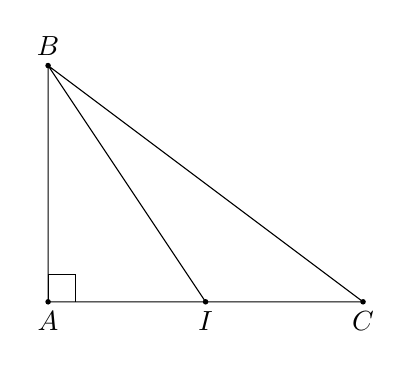
\begin{tikzpicture}[>=stealth,x=1cm,y=1cm,scale=1]
		\fill (0,3) circle (1pt) node[above]{$B$};
		\fill (4,0) circle (1pt) node[below]{$C$};
		\fill (0,0) circle (1pt) node[below]{$A$};
		\fill (2,0) circle (1pt) node[below]{$I$};
		\draw (0,3)--(0,0)--(4,0)--(0,3)--(2,0);
		\draw (0,0)--++(90:.35)--++(0:.35)--++(-90:.35);
	\end{tikzpicture}
	}
	}
\end{bt}
\begin{bt}%[0H3K2-4]%[Dự án đề kiểm tra HKI NH22-23- Nguyễn Văn Sang]%[THPT Đô Lương 1 - Nghệ An]
	Trong mặt phẳng toạ độ $Oxy$, cho ba điểm $A(5;3)$, $B(-1;5)$, $C(2;-1)$.
	\begin{enumerate}
		\item Tìm toạ độ điểm $D$ sao cho tứ giác $ABDC$ là hình bình hành.
		\item Tìm toạ độ chân đường cao $H$ kẻ từ $A$ xuống cạnh $BC$ của tam giác $ABC$.
	\end{enumerate}
	\loigiai{
	\immini
	{
	\begin{enumerate}
	\item Tìm toạ độ điểm $D$ sao cho tứ giác $ABDC$ là hình bình hành.\\
	Vì $ABDC$ là hình bình hành nên ta có
	\begin{eqnarray*}
		&&\overrightarrow{CD}=\overrightarrow{AB}\\
		&\Leftrightarrow& \left( x_D-x_C;y_D-y_C\right) =\left(x_B-x_A;y_B-y_A \right)\\
		&\Leftrightarrow&\heva{& x_D-2=-1-5 \\ & y_D+1=5-3}\\
		&\Leftrightarrow&\heva{& x_D=-4 \\ & y_D=1.} 
	\end{eqnarray*}
	Vậy toạ độ điểm $D(-4;1)$.
	\item Tìm toạ độ chân đường cao $H$.\\
	Gọi $H(x;y)$ là chân đường cao $H$ kẻ từ $A$ xuống cạnh $BC$.\\
	Ta có 
	\begin{eqnarray*}
		&&\heva{& \overrightarrow{AH}\cdot \overrightarrow{BC}=0 \\& \overrightarrow{BH}, \overrightarrow{BC} \text{ cùng phương}}
		\Leftrightarrow \heva{& \left(x-5;y-3\right)\cdot\left(3;-6\right)=0 \\& \left(x+1;y-5 \right) =k\left(3;-6\right) }\\
		&\Leftrightarrow& \heva{& 3x-15-6y+18=0\\&x+1=3k\\&y-5=-6k}	\Leftrightarrow \heva{& 3x-6y=-3\\&x-3k=-1\\&y+6k=5}\\
		&\Leftrightarrow& \heva{& x=1\\&y=1\\&k=\dfrac{2}{3}}\Rightarrow H(1;1).
	\end{eqnarray*}
	Vậy chân đường cao kẻ từ $A$ xuống cạnh $BC$ là $H(1;1)$.
	\end{enumerate}
	}
	{
	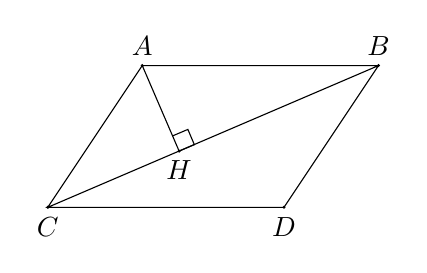
\begin{tikzpicture}[>=stealth,x=1cm,y=1cm,scale=.6]
		\fill (0,0) circle (1pt) node[below]{$C$};
		\fill (2,3) circle (1pt) node[above]{$A$};
		\fill (7,3) circle (1pt) node[above]{$B$};
		\fill (5,0) circle (1pt) node[below]{$D$};
		\fill (2.78,1.19) circle (1pt) node[below]{$H$};
		\draw (0,0)--(2,3)--(7,3)--(5,0)--(0,0)--(7,3) (2,3)--(2.78,1.19);
		\draw (2.78,1.19)--++(23:.35)--++(90+23:.35)--++(180+23:.35);
	\end{tikzpicture}
	}
	}
\end{bt}
\begin{bt}%[X1B4-1]%[Dự án đề kiểm tra HKI NH22-23- Nguyễn Văn Sang]%[THPT Đô Lương 1 - Nghệ An]
	Thu nhập theo tháng (đơn vị: triệu đồng) của các công nhân trong một công ty được cho như sau
	\begin{center}
		\begin{tabular}{|l|c|c|c|c|c|c|c|c|c|c|c|c|c|c|}
			\hline Thu nhập & 4{,}0 & 4{,}5 & 5{,}5 & 6{,}0 & 7{,}0 & 7{,}5 & 8{,}0 & 8{,}5 & 9{,}5 & 10 & 11 & 12 & 13 & \\
			\hline Tần số & 1 & 1 & 1 & 1 & 2 & 1 & 2 & 1 & 2 & 1 & 1 & 1 & 1 & $\mathrm{~N}=16$ \\
			\hline
		\end{tabular}
	\end{center}
\begin{enumerate}
	\item Tính thu nhập trung bình theo tháng của công nhân công ty.
	\item Trong đại dịch Covid-19 công ty có chính sách hỗ trợ $25\%$ công nhân có thu nhập thấp nhất. Số nào trong các tứ phân vị giúp xác định được các công nhân trong diện diện được hỗ trợ? Tính giá trị của tứ phân vị đó.
\end{enumerate}
	\loigiai{
		 Sắp xếp các số liệu theo thứ tự không giảm, ta được
		 $$4{,}0;4{,}5;5{,}5;6{,}0;7{,}0;7{,}0;7{,}5;8{,}0,8{,}0;8{,}5;9{,}5;9{,}5;10{,}0;11{,}0;12{,}0;13{,}0.$$
	\begin{enumerate}
		\item Tính thu nhập trung bình theo tháng của công nhân công ty.\\
		Cỡ mẫu là $N=16$.\\
		Đặt $A=4{,}0+4{,}5+5{,}5+6{,}0+7{,}0+7{,}0+7{,}5+8{,}0=49{,}5$.\\
		Đặt $B=8{,}0+8{,}5+9{,}5+9{,}5+10{,}0+11{,}0+12{,}0+13{,}0=81{,}5$.\\
		Số trung bình $\overline{x}=\dfrac{A+B}{16}=8{,}1875$.
		\item Trong đại dịch Covid-19 công ty có chính sách hỗ trợ $25\%$ công nhân có thu nhập thấp nhất. Số nào trong các tứ phân vị giúp xác định được các công nhân trong diện diện được hỗ trợ? Tính giá trị của tứ phân vị đó.\\
		Số thứ nhất trong các tứ phân vị giúp xác định được giới hạn dưới cho $25\%$ số công nhân có thu nhập thấp nhất được hỗ trợ.\\
		Vì cỡ mẫu là số chẵn nên trung vị mẫu là $\dfrac{8{,}0+8{,}0}{2}=8{,}0$.\\
		Tứ phân vị thứ hai là trung vị của mẫu số liệu đã cho nên $Q_2=8{,}0$.\\
		Tứ phân vị thứ nhất là trung vị của mẫu
		$$4{,}0;4{,}5;5{,}5;6{,}0;7{,}0;7{,}0;7{,}5;8{,}0$$
		Do đó $Q_1=6{,}5$.\\
		Vậy các giá trị của tứ phân vị thứ nhất là $4{,}0;4{,}5;5{,}5;6{,}0$.
	\end{enumerate}
	}
\end{bt}